\subsection{Timeline and Topic Bars}

\subsubsection{General}
The Timeline is our interface to control the time in \textsc{HistoGlobe}. It is located at the bottom. In the center on certain moment of history is displayed. With the plus and minus on the left you can zoom in and out. Tis is done by stretching and compressing the timeline. It is possible to chainge the actual date by pulling the timeline to left or right.

\begin{figure}[H]
	\centering
	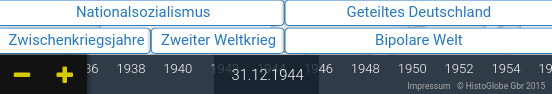
\includegraphics[width=0.8\textwidth]{graphics/timeline_now.png}
	\caption{Timeline}
\end{figure}

\subsubsection{Structure}
One requirement of the teacher is to present time in history not linear but in epochs. The advantage is that he can give focus to special subsets of history. In our implementation we have two different types of epoch bars: German history and world history.

So our actual implementation of the timeline consists of four layers. The top layer describes the German history from "Deutsches Kaiserreich" to "Geteiltes Deutschland". The next two layers belong together. They represent the world history. The upper of the two layers is only shown if one category of the world history is selected. Like in picture ~\ref{fig:Timeline_Elements}. Here "Imperialismus" is active and on top of this layer is the subtopic layer with specific topics. TimelineLayer

\begin{figure}[H]
	\centering
	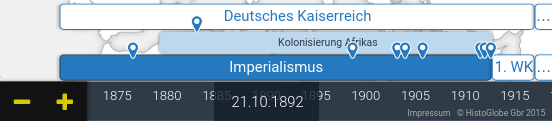
\includegraphics[width=0.8\textwidth]{graphics/timeline_elements.png}
	\caption{Timeline Elements}
	\label{fig:Timeline_Elements}
\end{figure}



\subsubsection{Behaviour}
Zooming 

Pulling 

Abkürzungen

Zentrierte Namen

Zentrierung der Zeit bei active

Hivents hoverbar und clickbar